\section{Généralités sur le cerveau}

Pour mieux comprendre l'aphasie en général et celle de Broca en particulier, 
il convient de commencer avec le cerveau et notamment les fonctions cognitives de communication. On voit la structure du cortex cérébral humain sur la Figure~\ref{fig:human-brain}.

\begin{figure}
    \begin{center}
        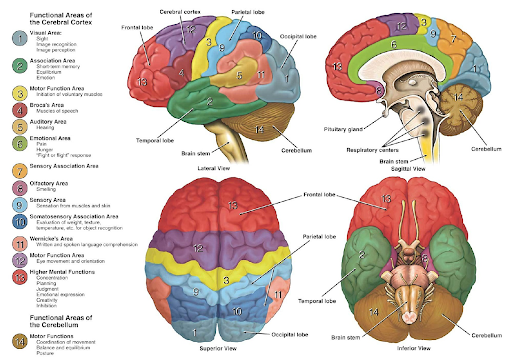
\includegraphics[width=\textwidth]{unnamed}
    \end{center}
    \caption{Structure du cerveau humain}
    \label{fig:human-brain}
\end{figure}

L'aphasie de Broca en particulier est causé par une lésion dans l'aire de Broca, typiquement suite à un AVC.